\begin{pages}
    \begin{Rightside}
    \selectlanguage{greek}
        \beginnumbering
        \pstart[
        			\chapter{Τὸ τὰς φιάλας ἐκχέαι}
        			\markboth{The Emptying of the Vials}
				]
		\renewcommand{\LettrineFontHook}{\PHtitl}
		\lettrine[lines=3]{Κ}{αὶ} ἤκουσα μεγάλης φωνῆς ἐκ τοῦ ναοῦ λεγούσης τοῖς ἑπτὰ ἀγγέλοις Ὑπάγετε καὶ ἐκχέετε τὰς ἑπτὰ φιάλας τοῦ θυμοῦ τοῦ Θεοῦ εἰς τὴν γῆν. Καὶ ἀπῆλθεν ὁ πρῶτος καὶ ἐξέχεεν τὴν φιάλην αὐτοῦ εἰς τὴν γῆν· καὶ ἐγένετο ἕλκος κακὸν καὶ πονηρὸν ἐπὶ τοὺς ἀνθρώπους τοὺς ἔχοντας τὸ χάραγμα τοῦ θηρίου καὶ τοὺς προσκυνοῦντας τῇ εἰκόνι αὐτοῦ. 
		\pend
		\pstart
		Καὶ ὁ δεύτερος ἐξέχεεν τὴν φιάλην αὐτοῦ εἰς τὴν θάλασσαν· καὶ ἐγένετο αἷμα ὡς νεκροῦ, καὶ πᾶσα ψυχὴ ζωῆς ἀπέθανεν, τὰ ἐν τῇ θαλάσσῃ. Καὶ ὁ τρίτος ἐξέχεεν τὴν φιάλην αὐτοῦ εἰς τοὺς ποταμοὺς καὶ τὰς πηγὰς τῶν ὑδάτων· καὶ ἐγένετο αἷμα. Καὶ ἤκουσα τοῦ ἀγγέλου τῶν ὑδάτων λέγοντος Δίκαιος εἶ, ὁ ὢν καὶ ὁ ἦν, ὁ Ὅσιος, ὅτι ταῦτα ἔκρινας, ὅτι αἷμα ἁγίων καὶ προφητῶν ἐξέχεαν, καὶ αἷμα αὐτοῖς δέδωκας πεῖν· ἄξιοί εἰσιν. 
		\pend
		\pstart
		Καὶ ἤκουσα τοῦ θυσιαστηρίου λέγοντος Ναί, Κύριε ὁ Θεός ὁ Παντοκράτωρ, ἀληθιναὶ καὶ δίκαιαι αἱ κρίσεις σου. Καὶ ὁ τέταρτος ἐξέχεεν τὴν φιάλην αὐτοῦ ἐπὶ τὸν ἥλιον· καὶ ἐδόθη αὐτῷ καυματίσαι τοὺς ἀνθρώπους ἐν πυρί. καὶ ἐκαυματίσθησαν οἱ ἄνθρωποι καῦμα μέγα, καὶ ἐβλασφήμησαν τὸ ὄνομα τοῦ Θεοῦ τοῦ ἔχοντος τὴν ἐξουσίαν ἐπὶ τὰς πληγὰς ταύτας, καὶ οὐ μετενόησαν δοῦναι αὐτῷ δόξαν. 
		\pend
		\pstart
		Καὶ ὁ πέμπτος ἐξέχεεν τὴν φιάλην αὐτοῦ ἐπὶ τὸν θρόνον τοῦ θηρίου· καὶ ἐγένετο ἡ βασιλεία αὐτοῦ ἐσκοτωμένη, καὶ ἐμασῶντο τὰς γλώσσας αὐτῶν ἐκ τοῦ πόνου, καὶ ἐβλασφήμησαν τὸν Θεὸν τοῦ οὐρανοῦ ἐκ τῶν πόνων αὐτῶν καὶ ἐκ τῶν ἑλκῶν αὐτῶν, καὶ οὐ μετενόησαν ἐκ τῶν ἔργων αὐτῶν. 
		\pend
		\pstart
		Καὶ ὁ ἕκτος ἐξέχεεν τὴν φιάλην αὐτοῦ ἐπὶ τὸν ποταμὸν τὸν μέγαν Εὐφράτην· καὶ ἐξηράνθη τὸ ὕδωρ αὐτοῦ, ἵνα ἑτοιμασθῇ ἡ ὁδὸς τῶν βασιλέων τῶν ἀπὸ ἀνατολῆς ἡλίου. Καὶ εἶδον ἐκ τοῦ στόματος τοῦ δράκοντος καὶ ἐκ τοῦ στόματος τοῦ θηρίου καὶ ἐκ τοῦ στόματος τοῦ ψευδοπροφήτου πνεύματα τρία ἀκάθαρτα ὡς βάτραχοι· εἰσὶν γὰρ πνεύματα δαιμονίων ποιοῦντα σημεῖα, ἃ ἐκπορεύεται ἐπὶ τοὺς βασιλεῖς τῆς οἰκουμένης ὅλης, συναγαγεῖν αὐτοὺς εἰς τὸν πόλεμον τῆς ἡμέρας τῆς μεγάλης τοῦ Θεοῦ τοῦ Παντοκράτορος. 
		\pend
		\pstart
		Ἰδοὺ ἔρχομαι ὡς κλέπτης· μακάριος ὁ γρηγορῶν καὶ τηρῶν τὰ ἱμάτια αὐτοῦ, ἵνα μὴ γυμνὸς περιπατῇ καὶ βλέπωσιν τὴν ἀσχημοσύνην αὐτοῦ. καὶ συνήγαγεν αὐτοὺς εἰς τὸν τόπον τὸν καλούμενον Ἑβραϊστὶ Ἁρμαγεδών. 
		\pend
		\pstart
		Καὶ ὁ ἕβδομος ἐξέχεεν τὴν φιάλην αὐτοῦ ἐπὶ τὸν ἀέρα· καὶ ἐξῆλθεν φωνὴ μεγάλη ἐκ τοῦ ναοῦ ἀπὸ τοῦ θρόνου λέγουσα Γέγονεν. καὶ ἐγένοντο ἀστραπαὶ καὶ φωναὶ καὶ βρονταί, καὶ σεισμὸς ἐγένετο μέγας, οἷος οὐκ ἐγένετο ἀφ’ οὗ ἄνθρωπος ἐγένετο ἐπὶ τῆς γῆς, τηλικοῦτος σεισμὸς οὕτω μέγας.
		\pend 
		\pstart
		καὶ ἐγένετο ἡ πόλις ἡ μεγάλη εἰς τρία μέρη, καὶ αἱ πόλεις τῶν ἐθνῶν ἔπεσαν. καὶ Βαβυλὼν ἡ μεγάλη ἐμνήσθη ἐνώπιον τοῦ Θεοῦ δοῦναι αὐτῇ τὸ ποτήριον τοῦ οἴνου τοῦ θυμοῦ τῆς ὀργῆς αὐτοῦ. καὶ πᾶσα νῆσος ἔφυγεν, καὶ ὄρη οὐχ εὑρέθησαν. 
		\pend
		\pstart
		καὶ χάλαζα μεγάλη ὡς ταλαντιαία καταβαίνει ἐκ τοῦ οὐρανοῦ ἐπὶ τοὺς ἀνθρώπους· καὶ ἐβλασφήμησαν οἱ ἄνθρωποι τὸν Θεὸν ἐκ τῆς πληγῆς τῆς χαλάζης, ὅτι μεγάλη ἐστὶν ἡ πληγὴ αὐτῆς σφόδρα.
		\pend
        \endnumbering
    \end{Rightside}
    \begin{Leftside}
        \beginnumbering
        \pstart[
        			\chapter{The Emptying of the Vials}
				]		
		\renewcommand{\LettrineFontHook}{\Zallmanfamily}
		\lettrine[lines=3]{A}{nd} I heard a great voice from the temple, telling the seven angels, “Arise and empty the seven vials of the wrath of God into the Earth.” And the first one left and emptied his vial into the Earth; and bad and painful sores befell (happened) the people having the mark of the beast and those worshipping its idol. 
		\pend
		\pstart
		And the second (one) emptied his vial into the sea; and it became blood, as that of a dead (person), and all living soul died, (at least) the ones in the sea. And the third (one) emptied his vial into into the rivers and the springs of waters — and they became blood. And I heard the angel of the waters saying, “You are just, (You) who is and who was (and) the Hallowed — (You are these things) for you have judged thus. For they poured out the blood of holy (men) and (that) of prophets; and blood (is what) You have given them to drink. (For) they are worthy.”
		\pend
		\pstart
		And I heard (someone from?) the altar saying, “Yes O Lord God, the Almighty, true and just are Your judgements.” And the fourth (one) emptied his vial upon the Sun; and there was given to him (the authority) to scorch (all) the humans in (with) fire. And the people were scorched (in, with) a great heat; and they blasphemed the name of God — the One having the authority over their plagues (sufferings). And they did not repent (of their sins) to give Him glory. 
		\pend
		\pstart
		And the fifth (one) emptied his vial onto the throne of the beast; and its kingdom was darkened (overshadowed) and they gnawed their tongues from (because of) the suffering (toil). And they blasphemed the God of Heaven from (because of) their suffering (toils) and from their sores; and they did not repent of their deeds. 
		\pend
		\pstart
		And the sixth (one) emptied his vial onto the great river (called) Euphrates; and its water dried up (withered) so that the path of the kings of the East might be prepared. And I saw three unclean spirits — like frogs — (coming) from the mouth of the dragon and from the mouth of the beast and from the mouth of the false prophet. For they are (the) spirits of demons, making signs, which come forth upon the kings of the entire (inhabited) world (and) to collect (gather) them (and lead them?) to the war of the great day of God the Almighty. 
		\pend
		\pstart
		Look, I am coming like a thief. Blessed is he who is watchful and (he who) keeps his garments (clean), so that he does not walk about naked and (so that) they might not see his shame. And he gathered them in(to) the region (that is) called Armageddon (lit. Harmagedon) in Hebrew. 
		\pend
		\pstart
		And the seventh (one) emptied his vial onto the air; and there came a great voice from the temple from the throne saying, “It has happened.” And there were (bolts of) lightning and voices and thunder and a great tremor occurred, such as has not happened since the time during which man appeared on the Earth — so great a tremor (occurred). 
		\pend
		\pstart
		And the great city was trisected (lit. it fell into three parts) and the cities of the nations fell. And the great Babylon was remembered before God (and He remembered) to give to Babylon the cup of the wine of His anger. And every island fled, and mountains were not (any longer) found (anywhere). 
		\pend
		\pstart
		And a great hail descended from Heaven upon the people (and each hailstone was, in weight) like a talent (approximately 60 kg). And the people blasphemed God from (because of) their suffering of the hail, for their sufferings are very great. 
		\pend
        \endnumbering
    \end{Leftside}

\end{pages} 
\Pages

\clearpage
\thispagestyle{empty}
\null\vfill
\settowidth\longest{\huge\itshape […] and when I turned around I saw}
\begin{center}
\parbox{\longest}{%
  \raggedright{\huge\itshape%
    ``And he gathered them in(to) the region (that is) called Armageddon […] '' \par\bigskip
  }
  \raggedleft\Large\MakeUppercase{``Armageddon'' — Nicholas Roerich, 1935}\par%
}
\vfill\vfill
\clearpage\newpage
\end{center}
\newpage
\thispagestyle{empty}
\begin{center}
	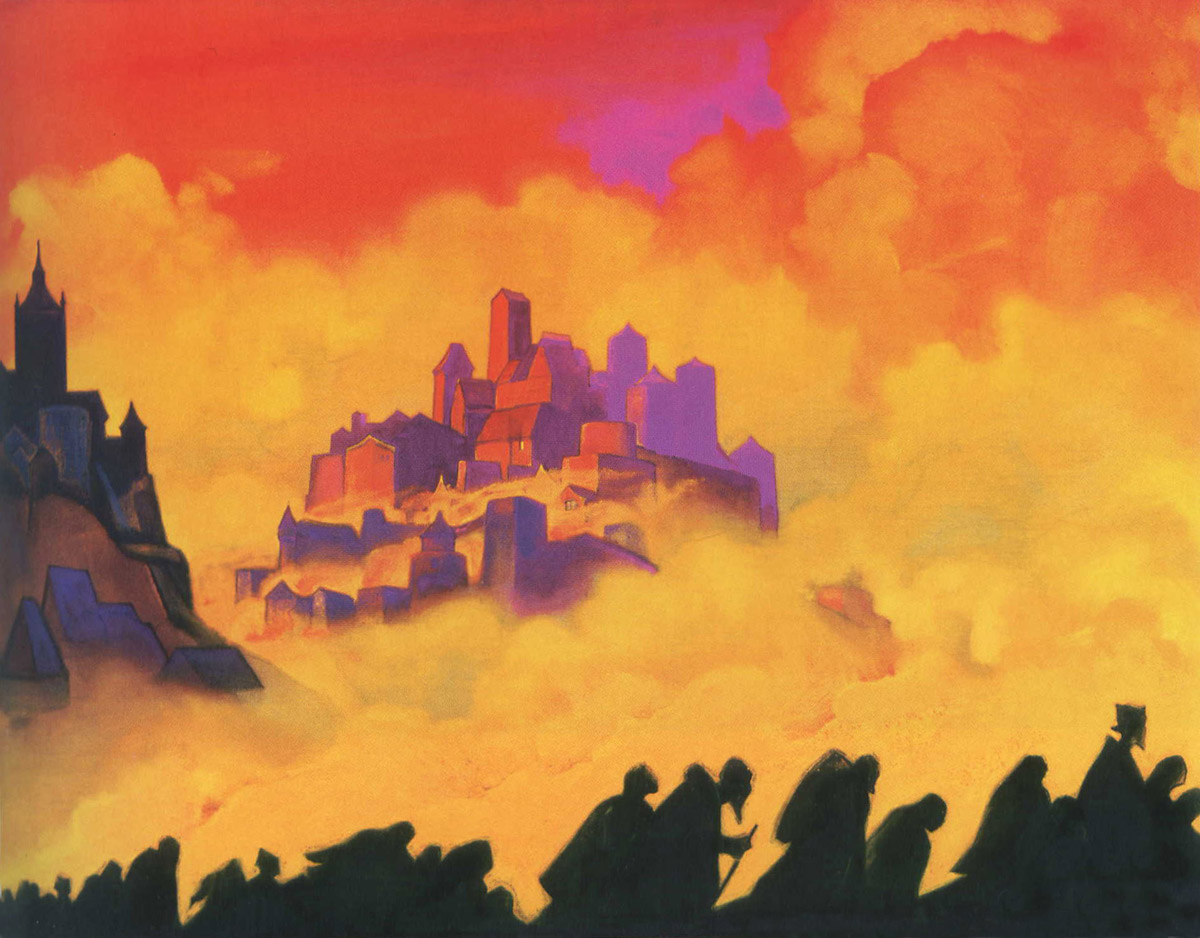
\includegraphics[angle=90, width=1\textwidth]{images/illustrations/roericharmageddon}
\end{center}